\documentclass{report}
\usepackage{luatexja} % LuaTeXで日本語を使うためのパッケージ
\usepackage{luatexja-fontspec} % LuaTeX用の日本語フォント設定

% --- 数学関連 ---
\usepackage{amsmath, amssymb, amsfonts, mathtools, bm, amsthm} % 基本的な数学パッケージ
\usepackage{type1cm, upgreek} % 数式フォントとギリシャ文字
\usepackage{physics, mhchem} % 物理や化学の記号や式の表記を簡単にする

% --- 表関連 ---
\usepackage{multirow, longtable, tabularx, array, colortbl, dcolumn, diagbox} % 表のレイアウトを柔軟にする
\usepackage{tablefootnote, truthtable} % 表中に注釈を追加、真理値表
\usepackage{tabularray} % 高度な表組みレイアウト

% --- グラフィック関連 ---
\usepackage{tikz, graphicx} % 図の描画と画像の挿入
\usepackage{background} % ウォーターマークの設定
\usepackage{caption, subcaption} % 図や表のキャプション設定
\usepackage{float, here} % 図や表の位置指定

% --- レイアウトとページ設定 ---
\usepackage{fancyhdr} % ページヘッダー、フッター、余白の設定
\usepackage[top = 20truemm, bottom = 20truemm, left = 20truemm, right = 20truemm]{geometry}
\usepackage{fancybox, ascmac} % ボックスのデザイン

% --- 色とスタイル ---
\usepackage{xcolor, color, colortbl, tcolorbox} % 色とカラーボックス
\usepackage{listings, jvlisting} % コードの色付けとフォーマット

% --- 参考文献関連 ---
\usepackage{biblatex, usebib} % 参考文献の管理と挿入
\usepackage{url, hyperref} % URLとリンクの設定

% --- その他の便利なパッケージ ---
\usepackage{footmisc} % 脚注のカスタマイズ
\usepackage{multicol} % 複数段組
\usepackage{comment} % コメントアウトの拡張
\usepackage{siunitx} % 単位の表記
\usepackage{docmute}
% \usepackage{appendix}
% --- tcolorboxとtikzの設定 ---
\tcbuselibrary{theorems, breakable} % 定理のボックスと改ページ設定
\usetikzlibrary{decorations.markings, arrows.meta, calc} % tikzの装飾や矢印の設定

% --- 定理スタイルと数式設定 ---
\theoremstyle{definition} % 定義スタイル
\numberwithin{equation}{section} % 式番号をサブセクション単位でリセット

% --- hyperrefの設定 ---
\hypersetup{
  setpagesize = false,
  bookmarks = true,
  bookmarksdepth = tocdepth,
  bookmarksnumbered = true,
  colorlinks = false,
  pdftitle = {}, % PDFタイトル
  pdfsubject = {}, % PDFサブジェクト
  pdfauthor = {}, % PDF作者
  pdfkeywords = {} % PDFキーワード
}

% --- siunitxの設定 ---
\sisetup{
  table-format = 1.5, % 小数点以下の桁数
  table-number-alignment = center, % 数値の中央揃え
}

% --- 透かし画像の設定 --- 
\backgroundsetup{
  scale=0.5,                       % 画像のスケール
  % color=black,                   % 画像の色(透かし用に半透明が推奨)
  opacity=0.2,                   % 透かしの透明度(0が完全透明、1が完全不透明)
  angle=0,                       % 画像の角度
  position = current page.south east,  % ページの右下
  hshift=-6cm, % 右方向へのシフト(負の値で内側に移動)
  vshift=5cm,  % 上方向へのシフト(正の値で内側に移動)
  contents={
\includegraphics{./fig/appilogo-circular-full.png}} % 画像のパス
}

% --- その他の設定 ---
\allowdisplaybreaks % 数式の途中改ページ許可
\newcolumntype{t}{!{\vrule width 0.1pt}} % 新しいカラムタイプ
\newcolumntype{b}{!{\vrule width 1.5pt}} % 太いカラム
\UseTblrLibrary{amsmath, booktabs, counter, diagbox, functional, hook, html, nameref, siunitx, varwidth, zref} % tabularrayのライブラリ
\setlength{\columnseprule}{0.4pt} % カラム区切り線の太さ
\captionsetup[figure]{font = bf} % 図のキャプションの太字設定
\captionsetup[table]{font = bf} % 表のキャプションの太字設定
\captionsetup[lstlisting]{font = bf} % コードのキャプションの太字設定
\captionsetup[subfigure]{font = bf, labelformat = simple} % サブ図のキャプション設定
\setcounter{secnumdepth}{4} % セクションの深さ設定
\newcolumntype{d}{D{.}{.}{5}} % 数値のカラム
\newcolumntype{M}[1]{>{\centering\arraybackslash}m{#1}} % センター揃えのカラム
\DeclareMathOperator{\diag}{diag}
\everymath{\displaystyle} % 数式のスタイル
\newcommand{\inner}[2]{\left\langle #1, #2 \right\rangle}
\renewcommand{\figurename}{図}
\renewcommand{\i}{\mathrm{i}} % 複素数単位i
\renewcommand{\laplacian}{\grad^2} % ラプラシアンの記号
\renewcommand{\thesubfigure}{(\alph{subfigure})} % サブ図の番号形式
\newcommand{\m}[3]{\multicolumn{#1}{#2}{#3}} % マルチカラムのショートカット
\renewcommand{\r}[1]{\mathrm{#1}} % mathrmのショートカット
\newcommand{\e}{\mathrm{e}} % 自然対数の底e
\newcommand{\Ef}{E_{\mathrm{F}}} % フェルミエネルギー
\renewcommand{\c}{\si{\degreeCelsius}} % 摂氏記号
\renewcommand{\d}{\r{d}} % d記号
\renewcommand{\t}[1]{\texttt{#1}} % タイプライタフォント
\newcommand{\kb}{k_{\mathrm{B}}} % ボルツマン定数
% \renewcommand{\phi}{\varphi} % ϕをφに変更
\renewcommand{\epsilon}{\varepsilon}
\newcommand{\fullref}[1]{\textbf{\ref{#1} \nameref{#1}}}
\newcommand{\reff}[1]{\textbf{図\ref{#1}}} % 図参照のショートカット
\newcommand{\reft}[1]{\textbf{表\ref{#1}}} % 表参照のショートカット
\newcommand{\refe}[1]{\textbf{式\eqref{#1}}} % 式参照のショートカット
\newcommand{\refp}[1]{\textbf{コード\ref{#1}}} % コード参照のショートカット
\renewcommand{\lstlistingname}{コード} % コードリストの名前
\renewcommand{\theequation}{\thesection.\arabic{equation}} % 式番号の形式
\renewcommand{\footrulewidth}{0.4pt} % フッターの線
\newcommand{\mar}[1]{\textcircled{\scriptsize #1}} % 丸囲み文字
\newcommand{\combination}[2]{{}_{#1} \mathrm{C}_{#2}} % 組み合わせ
\newcommand{\thline}{\noalign{\hrule height 0.1pt}} % 細い横線
\newcommand{\bhline}{\noalign{\hrule height 1.5pt}} % 太い横線

% --- カスタム色定義 ---
\definecolor{burgundy}{rgb}{0.5, 0.0, 0.13} % バーガンディ色
\definecolor{charcoal}{rgb}{0.21, 0.27, 0.31} % チャコール色
\definecolor{forest}{rgb}{0.0, 0.35, 0} % 森の緑色

% --- カスタム定理環境の定義 ---
\newtcbtheorem[number within = chapter]{myexc}{練習問題}{
  fonttitle = \gtfamily\sffamily\bfseries\upshape,
  colframe = forest,
  colback = forest!2!white,
  rightrule = 1pt,
  leftrule = 1pt,
  bottomrule = 2pt,
  colbacktitle = forest,
  theorem style = standard,
  breakable,
  arc = 0pt,
}{exc-ref}
\newtcbtheorem[number within = chapter]{myprop}{命題}{
  fonttitle = \gtfamily\sffamily\bfseries\upshape,
  colframe = blue!50!black,
  colback = blue!50!black!2!white,
  rightrule = 1pt,
  leftrule = 1pt,
  bottomrule = 2pt,
  colbacktitle = blue!50!black,
  theorem style = standard,
  breakable,
  arc = 0pt
}{proposition-ref}
\newtcbtheorem[number within = chapter]{myrem}{注意}{
  fonttitle = \gtfamily\sffamily\bfseries\upshape,
  colframe = yellow!20!black,
  colback = yellow!50,
  rightrule = 1pt,
  leftrule = 1pt,
  bottomrule = 2pt,
  colbacktitle = yellow!20!black,
  theorem style = standard,
  breakable,
  arc = 0pt
}{remark-ref}
\newtcbtheorem[number within = chapter]{myex}{例題}{
  fonttitle = \gtfamily\sffamily\bfseries\upshape,
  colframe = black,
  colback = white,
  rightrule = 1pt,
  leftrule = 1pt,
  bottomrule = 2pt,
  colbacktitle = black,
  theorem style = standard,
  breakable,
  arc = 0pt
}{example-ref}
\newtcbtheorem[number within = chapter]{exc}{Requirement}{myexc}{exc-ref}
\newcommand{\rqref}[1]{{\bfseries\sffamily 練習問題 \ref{exc-ref:#1}}}
\newtcbtheorem[number within = chapter]{definition}{Definition}{mydef}{definition-ref}
\newcommand{\dfref}[1]{{\bfseries\sffamily 定義 \ref{definition-ref:#1}}}
\newtcbtheorem[number within = chapter]{prop}{命題}{myprop}{proposition-ref}
\newcommand{\prref}[1]{{\bfseries\sffamily 命題 \ref{proposition-ref:#1}}}
\newtcbtheorem[number within = chapter]{rem}{注意}{myrem}{remark-ref}
\newcommand{\rmref}[1]{{\bfseries\sffamily 注意 \ref{remark-ref:#1}}}
\newtcbtheorem[number within = chapter]{ex}{例題}{myex}{example-ref}
\newcommand{\exref}[1]{{\bfseries\sffamily 例題 \ref{example-ref:#1}}}
% --- 再定義コマンド ---
% \mathtoolsset{showonlyrefs=true} % 必要な式番号のみ表示
\pagestyle{fancy} % ヘッダー・フッターのスタイル設定
\chead{応用量子物性講義ノート} % 中央ヘッダー
% \rhead{}
\fancyhead[R]{\rightmark}
\renewcommand{\sectionmark}[1]{\markright{\thesection\ #1}}
\cfoot{\thepage} % 中央フッターにページ番号
\lhead{}
\rfoot{Yuto Masuda and Haruki Aoki} % 右フッターに名前
\setcounter{tocdepth}{4} % 目次の深さ
\makeatletter
\@addtoreset{equation}{section} % サブセクションごとに式番号をリセット
\makeatother

% --- メタ情報 ---
\title{応用量子物性講義ノート}
\date{更新日\today}
\author{Yuto Masuda and Haruki Aoki}

\begin{document}
  一般に,散乱の波動関数は,
  \begin{align}
    \psi(\bm{r}) = \e^{\i kz} + \int G_0 (\bm{r} - \bm{r'}) \frac{2m}{\hbar^2} V(\bm{r'}) \psi(\bm{r'}) \dd{\bm{r'}}\label{wave-funtion-of-scattering}
  \end{align}
  と表されるのであった.
  この波動関数を厳密に求めることは困難であるため近似を考える.
  まず,\refe{wave-funtion-of-scattering}を簡略化して,
  \begin{align}
    \psi(\bm{r}) = \psi_0 + \int g V \psi(\bm{r}') \dd{\bm{r}'}\label{simple-wave-funtion-of-scattering}
  \end{align}
  と表現する.
  ただし,
  \begin{align}
    g(\bm{r}) \coloneqq G_0(\bm{r})\frac{2m}{\hbar^2}
  \end{align}
  である.
  \refe{simple-wave-funtion-of-scattering}を再帰的に代入すると,
  \begin{align}
    \psi(\bm{r}) &= \psi_0 + \int g V \psi(\bm{r'}) \dd{\bm{r'}} \\
    &= \psi_0 + \int gV \qty(\psi_0 + \int g V \psi(\bm{r''}) \dd{\bm{r''}}) \dd{\bm{r'}} \\
    &= \psi_0 + \int g V \psi_0(\bm{r'}) \dd{\bm{r'}} + \iint gVgV \psi(\bm{r''}) \dd{\bm{r'}} \dd{\bm{r''}} \\
    &= \psi_0 + \int g V \psi_0(\bm{r'}) \dd{\bm{r'}} + \iint gVgV \psi_0(\bm{r''}) \dd{\bm{r'}} \dd{\bm{r''}} + \iiint gVgVgV \psi_0(\bm{r'''}) \dd{\bm{r'}} \dd{\bm{r''}} \dd{\bm{r'''}} + \cdots\label{dozens-of-gv}
  \end{align}
  を得る.
  \refe{dozens-of-gv}を第1項までで近似して,残りの項を捨てる.
  これは散乱の波動関数を平面波で近似することに相当する.
  つまり,
  \begin{align}
    \psi \simeq \psi_0
  \end{align}
  とする.これを\textbf{第1 Born近似}という\footnote{Max Born(1882-1970)}\footnote{砂川,散乱の量子論,
  「第1 Born近似がとくによく利用される理由は,何といってもその簡単さにある.したがって,ある散乱問題を手がけたとき,だれもが最初に試してみるのが,この近似である.
  そして思わしい結果がえられないとき,他の近似法を考えるのである.」}.
  \par
  Born近似を用いて散乱振幅を求める.$\bm{k} \coloneqq k\bm{e}_z$,$\bm{r} \coloneqq z\bm{e}_z$とすると,
  $\psi(\bm{r}') = \e^{\i \bm{k}\cdot\bm{r}'}$となるから,
  \begin{align}
    f^{(1)}(\theta) &= -\frac{1}{4\pi} \int \e^{\i \bm{k'}\cdot\bm{r'}} \frac{2m}{\hbar} V(\bm{r'}) \psi(\bm{r'}) \dd{\bm{r'}} \\
    &= -\frac{1}{4\pi}\frac{2m}{\hbar^2}\int\e^{-\i (\bm{k'} - \bm{k})\cdot\bm{r}'} V(\bm{r'}) \dd{\bm{r}'} \\
    &= -\frac{1}{4\pi}\frac{2m}{\hbar^2}\int\e^{-\i \bm{q} \cdot \bm{r}'} V(\bm{r'}) \dd{\bm{r}'}\label{potential-fourier-transform}
  \end{align}
  となる.ただし,散乱による運動量変化に対応する物理量を$\bm{q} \coloneqq \bm{k'} - \bm{k}$と定義した.
  \refe{potential-fourier-transform}を見ると,散乱振幅はポテンシャル$V(r)$のFourier変換から得られることがわかる\footnote{
    $f^{(n)}$は第$n$ Born近似による散乱振幅を意味する.
  }.
  また,球対称ポテンシャルのとき\refe{potential-fourier-transform}は簡略化できて,$V(\bm{r'}) \to V(r')$としてよいから,
  \begin{align}
    f^{(1)}(\theta) &= -\frac{1}{4\pi}\frac{2m}{\hbar^2}\int\e^{-\i \bm{q}\cdot \bm{r}'} V(r') \dd{\bm{r}'}\\
    &= -\frac{1}{4\pi}\frac{2m}{\hbar^2} \int_{\phi' = 0}^{2\pi}\dd{\phi'} \int_{\theta' = 0}^{\pi}\dd{\theta'}\int_{r' = 0}^{\infty}r'^2 \sin\theta' \dd{r'} \e^{-\i qr' \cos\theta'} V(r') \\
    &= -\frac{1}{4\pi}\frac{2m}{\hbar^2} 2\pi \int_{r' = 0}^{\infty}V(r')r'^2\int_{\theta' = 0}^{\pi} \e^{-\i qr' \cos\theta'} \sin\theta' \dd{r'}\dd{\theta'} \\ 
    &= -\frac{m}{\hbar^2} \int_{0}^{\infty} r'^2V(r') \frac{\e^{\i qr'} - \e^{-\i qr'}}{\i qr'} \dd{r'} \\ 
    &= -\frac{m}{\hbar^2} \int_{0}^{\infty} rV(r) \frac{\e^{\i qr} - \e^{-\i qr}}{\i q} \dd{r} \\ 
    &= -\frac{2m}{\hbar^2 q} \int_{0}^{\infty} rV(r)\sin\qty(qr) \dd{r}
  \end{align}
  となる.
  \begin{itembox}[l]{球対称ポテンシャルの散乱振幅}
    \begin{align}
      f^{(1)}(\theta) &= -\frac{m}{\hbar^2} \int_{0}^{\infty} rV(r) \frac{\e^{\i qr} - \e^{-\i qr}}{\i q} \dd{r}\label{SCamp1st-exp} \\ 
      &= -\frac{2m}{\hbar^2 q} \int_{0}^{\infty} rV(r)\sin\qty(qr) \dd{r}\label{SCamp1st-sin}
    \end{align}
  \end{itembox}
  \begin{myex}{湯川ポテンシャル}{}
    球対称ポテンシャル$V(r)$が,湯川ポテンシャルの場合を考える.
    湯川ポテンシャルは,
    \begin{align}
      V(r) = V_0 \frac{\e^{-\mu r}}{\mu r}
    \end{align}
    と書ける.
    による散乱を考える\footnote{湯川秀樹(1907-1981)}.これは,$V(r)$の到達距離が$\mu^{-1}$ほどであり,核子同士に働く力を表す.
    物質中では,伝導電子に遮蔽された不純物のCoulombポテンシャルを表す.
    $\mu = 1,2$及びCoulombポテンシャルのグラフを\reff{yukawa-potential-graph}に示す.
    このポテンシャルの下で散乱振幅$f^{(1)}(\theta)$と散乱断面積$\sigma^{(1)}(\theta)$を求めよ.
    \tcblower
    散乱振幅は\refe{SCamp1st-exp}より,
    \begin{align}
      f^{(1)}(\theta) &= -\frac{m}{\hbar^2} \int_{0}^{\infty} rV(r) \frac{\e^{\i qr} - \e^{-\i qr}}{\i q} \dd{r} \\ 
      &= -\frac{m}{\i \hbar^2 q \mu} \int_{0}^{\infty} rV_0\frac{e^{-\mu r}}{\mu r} \frac{\e^{\i qr} - \e^{-\i qr}}{\i q}\dd{r} \\
      &= -\frac{mV_0}{\i \hbar^2 q \mu} \int_{0}^{\infty} \qty[\exp\qty{(-\mu + \i q)r} - \exp\qty{(-\mu - \i q)r}] \dd{r} \\
      &= - \frac{2m V_0}{\hbar^2 \mu} \frac{1}{\mu^2 + q^2}
    \end{align}
    \par
    散乱振幅は,
    \begin{align}
      \sigma^{(1)}(\theta) &= \abs{f^{(1)}(\theta)}^2\\
      &= \qty(\frac{2m V_0}{\hbar^2 \mu})^2 \frac{1}{(\mu^2 + q^2)^2}\\
      &= \qty(\frac{2m V_0}{\hbar^2 \mu})^2 \frac{1}{\qty[\mu^2 + 4k^2 \sin^2\qty(\theta/2)]^2}
    \end{align}
    である.なお,$\bm{k'}$と$\bm{k}$のなす角が$\theta$であるので余弦定理より,$q = 2k\sin\theta/2$であることを用いた.
    \begin{figure}[H]
      \centering
      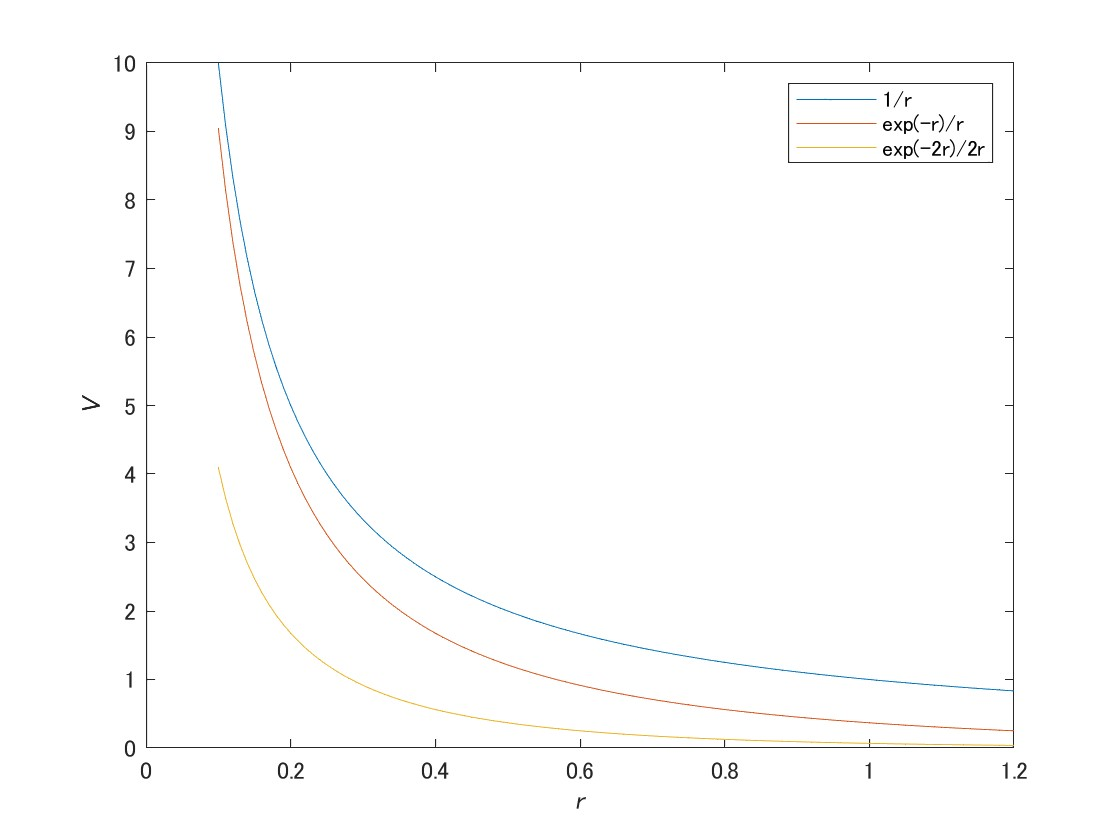
\includegraphics[width = 0.5\columnwidth]{fig/yukawa_potential.jpg}
      \caption{湯川ポテンシャルとCoulombポテンシャルの比較}\label{yukawa-potential-graph}
    \end{figure}
  \end{myex}
  \begin{myex}{Rutherford散乱(Griffith Example 10.6)}{}
    湯川ポテンシャルで$V_0 = \frac{q_1q_2}{4\pi \epsilon_0}$,$\mu = 0$とするとCoulombポテンシャル
    \begin{align}
      V(r) = \frac{q_1q_2}{4\pi\epsilon_0}
    \end{align}
    と一致する.\refe{SCamp1st-sin}に代入して散乱振幅を求める.
    \begin{align}
      f(\theta) &= - \frac{2m}{\hbar^2q} \int_{0}^{\infty} r \frac{q_1q_2}{4\pi\epsilon_0 r} \sin\qty(qr) \dd{r}\\
      &= -\frac{2m}{\hbar^2q}\frac{q_1q_2}{4\pi\epsilon_0}\int_{0}^{\infty} \sin\qty(qr) \dd{r} \\
      &=  -\frac{2m}{\hbar^2q}\frac{q_1q_2}{4\pi\epsilon_0}\qty(-\frac{1}{q}\qty[\cos\qty(qr)]_0^{\infty})\\
      &\simeq - \frac{mq_1q_1}{2\pi\epsilon_0\hbar^2q^2}\\
      &= - \frac{mq_1q_1}{8\pi\epsilon_0\hbar^2 \sin^2 \theta/2}
    \end{align}
  \end{myex}
\end{document}